\documentclass{article}



\usepackage{arxiv}

\usepackage[utf8]{inputenc} % allow utf-8 input
\usepackage[T1]{fontenc}    % use 8-bit T1 fonts
\usepackage{hyperref}       % hyperlinks
\usepackage{url}            % simple URL typesetting
\usepackage{booktabs}       % professional-quality tables
\usepackage{amsfonts}       % blackboard math symbols
\usepackage{nicefrac}       % compact symbols for 1/2, etc.
\usepackage{microtype}      % microtypography
\usepackage{lipsum}		% Can be removed after putting your text content
\usepackage{graphicx}
\usepackage{natbib}
\usepackage{doi}

\newcommand{\orcid}[1]{\href{https://orcid.org/#1}{\textcolor[HTML]{A6CE39}{\aiOrcid}}}


\title{DeepBucketLab - A playground for understanding deep learning for hydrologic process representations}

%\date{September 9, 1985}	% Here you can change the date presented in the paper title
%\date{} 					% Or removing it

\author{ 
    %\orcid{0000-0002-2533-3843}
    Jonathan M.~Frame \\
	Lynker Technologies\\
	Santa Barbara, CA 93103 \\
	\texttt{jframe@lynker.com} \\
	%% examples of more authors
	\And
    Leila ~Hernandez Rodriguez\\
	Lawrence Berkeley National Laboratory\\
	Berkeley, CA 94720 \\
	%\texttt{lchernandezrodriguez@lbl.gov} \\
	\And
    %\orcid{0000-0001-5795-9894}
    Maoya ~Bassiouni \\
    Environmental Science, Policy & Management\\
	University of California, Berkeley\\
	Berkeley, CA 94720 \\
	%\texttt{maoya@berkeley.edu} \\
}

% Uncomment to remove the date
%\date{}

% Uncomment to override  the `A preprint' in the header
%\renewcommand{\headeright}{Technical Report}
%\renewcommand{\undertitle}{Technical Report}
\renewcommand{\shorttitle}{\textit{arXiv} Template}

%%% Add PDF metadata to help others organize their library
%%% Once the PDF is generated, you can check the metadata with
%%% $ pdfinfo template.pdf
\hypersetup{
pdftitle={A template for the arxiv style},
pdfsubject={q-bio.NC, q-bio.QM},
pdfauthor={David S.~Hippocampus, Elias D.~Striatum},
pdfkeywords={First keyword, Second keyword, More},
}

\begin{document}
\maketitle
\begin{abstract}
Neural network-based models are currently state-of-the-art for predicting current and future hydrological conditions. Formal training in neural networks at the upper division and graduate levels of hydrology education is essential. We present a hands-on modeling tool for students in civil engineering and Earth science disciplines. This tool is designed to help them learn the fundamentals of neural network methods for dynamic systems modeling, with a particular emphasis on hydrological processes, and to practice conceptual thinking in training an effective neural network model for hydrological prediction.
\end{abstract}

% keywords can be removed
\keywords{Hydrologic modeling \and Neural networks \and Deep learning}

\section{Introduction}
Neural network-based modeling is becoming an essential component for water resources and environmental engineers and scientists, yet it is not sufficiently represented as a formal topic in current curricula. The need for Earth scientists, particularly hydrologists, to embrace deep learning as a critical component of natural systems modeling is well recognized \citep{nearing2021role}. Modeling as a formal topic in hydrology education has been championed by researchers who emphasize the critical role of simulation models in transforming the future of hydrologic and engineering education \citealp{aghakouchak2010application, aghakouchak2013educational}. As advancements have moved beyond simple conceptual models, it is crucial for university programs to embrace and teach these new methods.

With the increasing availability of hydrologic data over a wide range of scales, such as from remote sensing platforms, hydrology education has adopted simulation models to aid in understanding the complex behavior of hydrologic systems. However, recent results from the deep learning literature suggest that much of the traditional hydrological conceptual framework is misguided \citep{frame2023massbalance}. While neural networks and other ML methods have been in place in hydrology and water resources management for many years, the application of Machine Learning (ML), particularly Deep Learning (DL) models, has recently become widespread in hydrological modeling. This includes applications in rainfall-runoff modeling \citep{kratzert2018rainfall}, learning multi-scale hydrological behaviors \citep{kratzert2019towards}, and improving hydrologic predictions in ungauged basins \citep{kratzert2019towards}.

Various methods have been used to teach hydrological processes and modeling. \cite{aghakouchak2010application} applied a hands-on modeling tool (using a conceptual hydrological model) for training engineering students. A similar training tool with a Matlab Graphical User Interface (GUI) was developed and tested as a complement to theoretical hydrology lectures \citep{aghakouchak2013educational}. Sandtank-ML, a training tool at the interface of hydrology and ML, was recently published with a focus on subsurface hydrology \citep{gallagher2021sandtank}. While elaborate user interfaces are beneficial for building general intuition about some processes, they can separate users from the actual scientific methods used in modeling. Hydrological science is evolving towards a future likely to be dominated by a mix of AI and physics-based approaches. It is imperative that hydrologists do not perceive ML as merely another modeling toolbox. Instead, a comprehensive understanding of ML approaches, starting from the fundamental data science that drives these approaches, should be prioritized. Therefore, we have not used any interface to conceal our codes from the hydrology students and trainees who will be using them.

In this study, we test the use of a simplified deep learning model to provide students with first-hand experience of how and why deep learning is so effective at simulating complex hydrological processes. The model, described in the following section, is provided in a Python Notebook, allowing students to easily change the data, model hyperparameters, model architecture, etc., and observe their effects on the model's ability to learn a general hydrologic response (the general solution to the leaking bucket problem). This also enables students to run simple experiments testing various aspects of the pipeline, from data quality to model selection and performance metrics. This open-source, hands-on tool is developed for both undergraduate and graduate students to help them learn the fundamentals of deep learning for representing hydrologic processes and to adopt learning-based thinking in solving hydrologic engineering problems.

% ---------- % ---------- % ---------- % ---------- %
% ---------- % ---------- % ---------- % ---------- %
% ---------- % ---------- % ---------- % ---------- %
\section{Methods}
\label{sec:Methods}

We have developed a standalone Python-based notebook that guides students through every step of the modeling process, from data acquisition to model implementation, and finally to output and performance analysis. For this project, we opted for a synthetic data experiment to ensure that students can observe each aspect of the information flow, from data acquisition to the final results. Additionally, we provide references to well-documented examples using real-world data, available from a comprehensive neural network package designed for hydrologic simulations.

\subsection{Leaking Buckets as an Example of a "Hydrologic" System}
In DeepBucketLab, we demonstrate a general "bucket-style" model based on Torricelli's Law, which describes the outflow from a cylindrical tank:
\begin{equation}
\label{eq:torr}
\frac{dh}{dt} = A\sqrt{2gh}
\end{equation}
Here, the change in water height (h) is proportional to the square root of the water height, multiplied by a constant factor, in this case, the area of the spigot (A). We model the addition of mass to the bucket from the top as an open reservoir and the removal of mass through a spigot, which facilitates both upward and downward movement of water, represented as the head above the bucket bottom. Figure \ref{fig:schematic} presents a complete schematic of an individual bucket system.

\begin{figure}[h]
\centering
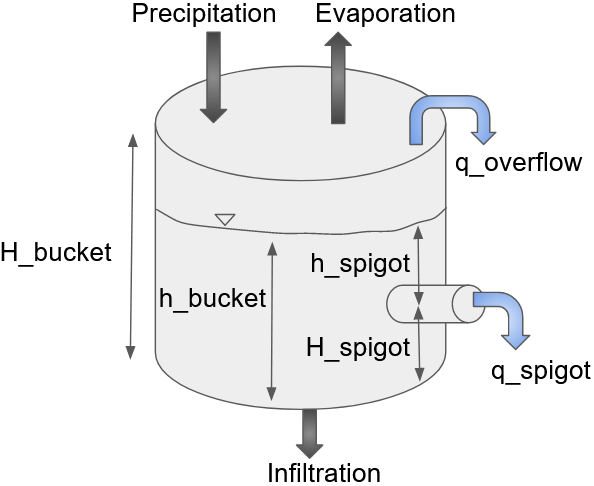
\includegraphics[width=\textwidth]{figures/bucket_schematic.png}
\caption{Schematic of the bucket model}
\label{fig:schematic}
\end{figure}

We define a bucket with five controlling attributes: the height of the bucket from bottom to rim, the height of the spigot from the bottom, a pseudo-infiltration parameter, the cross-sectional area of the bucket cylinder, and the cross-sectional area of the spigot. The primary objective of the neural network is to simulate the fluxes from the spigot  (Q\_spigot) and over the top of the bucket (Q\_overflow).

% ---------- % ---------- % ---------- % ---------- %
\subsubsection{Notebook environment with standard libraries}
We chose to develop this training in a stand alone Jupyter Notebook running Python. We include the minimal amount of standard libraries necessary. Numpy is a library for efficient vector calculations. Pandas is designed to easily store and access data, and it also comes with easy to impliment data transformation tools.
Matplotlip is a library that includes plotting functions. Torch is the main library for training the neural network. SciKitLearn is a package that helps prepare the data for training and analysis. tqdm displays the progress of the model training.

% ---------- % ---------- % ---------- % ---------- %
\subsubsection{Global constants, variables and model parameters}
\label{methods:parameters}
At the outset of the notebook, we declare a series of variables that govern every aspect of the model. These include both physical parameters, such as the gravitational constant, and numerical variables, like the computational time step, which are essential for generating the synthetic data that the Neural Network represents.

We define a certain number of subsystems (individual buckets) to train, validate, and test our model, along with specific time splits. These parameters are adjustable, allowing us to experiment with the amount of training data needed to generalize the model effectively across various leaking bucket scenarios.

Additionally, we include variables that are more appropriately described in the context of their specific roles within the model. These encompass parameters used in creating synthetic precipitation data, the static characteristics of the buckets, the level of noise added to the data, and the hyperparameters of the model. Each of these elements plays a crucial role in shaping the model's behavior and its ability to accurately simulate hydrological processes.

% ---------- % ---------- % ---------- % ---------- %
\subsubsection{Derived lists and values for setting up the splits in the data}
A critical aspect of training and utilizing a neural network is the selection and preparation of the data. We approach data splitting in two distinct ways to ensure robust model training and versatile application:

\begin{enumerate}

\item \textbf{Diversity in Training Systems}: We train the model on a sufficiently diverse range of systems. This diversity is key to developing a general model capable of accurately representing any random system. By incorporating a wide array of system types in the training data, we aim to create a model that is not limited to specific scenarios but can adapt to various conditions.

\item \textbf{Timing of Training Data}: The temporal aspect of the training data is equally important. We aim to avoid training the model exclusively on data from specific time periods that might not generalize well to other conditions. For example, a model trained solely during a drought period may not perform effectively in predicting conditions during periods of extreme precipitation.

\end{enumerate}

The overarching goal is to train a model that can accurately represent any type of leaking bucket within the predefined specifications. These specifications include variables such as the height and diameter of the bucket, the dimensions of the spigot, and certain types of losses that are deterministic yet difficult to measure directly. It's important to note that these bucket characteristics are conceptual and are not intended to directly represent real-world hydrologic systems. Instead, they serve as a simplified framework to facilitate the understanding and application of neural network modeling in hydrological contexts.

% ---------- % ---------- % ---------- % ---------- %
\subsubsection{Variations on the system inputs, creating the synthetic "precipitation"}
\label{methods:synthetic_inputs}
In our model, we modify two key aspects of the system to generate unique "hydrologic" responses, specifically focusing on simulating realistic precipitation trends. These modifications allow us to create diverse scenarios for the model to learn and predict.

The precipitation data, assumed to fill the bucket from the top, are generated through a stochastic process. This process is designed to mimic natural precipitation patterns and includes three distinct modes of precipitation, each occurring with different probabilities:

\begin{enumerate}
\item \textbf{No Precipitation}: Represents periods with no rainfall.
\item \textbf{Light Precipitation}: Characterized by frequent occurrences but with low magnitude.
\item \textbf{Heavy Precipitation}: Less frequent but with higher magnitude.
\end{enumerate}

Both low and heavy precipitation magnitudes are sampled from a uniform distribution within pre-defined ranges. Each realization of this stochastic process incorporates fixed probabilities for each of the precipitation modes and fixed ranges for precipitation magnitudes. This approach allows us to capture variations in climatological attributes, thereby providing a realistic and varied dataset for training the neural network.

% ---------- % ---------- % ---------- % ---------- %
\subsubsection{Bucket model numerical simulations as "ground truth"}
\label{methods:ground_truth}
To establish a reliable "ground truth" for our model, we conduct numerical simulations of the individual leaking buckets using the synthetic precipitation data. These simulations are crucial for training and validating the neural network, as they provide a benchmark against which the model's predictions can be compared.

The response of each bucket to the synthetic precipitation is simulated using Torricelli's Law, as described in Equation \ref{eq:torr}. This process involves calculating the change in water height within each bucket over time, considering the inflow from precipitation and the outflow through the spigot. By running these simulations, we generate a comprehensive dataset that captures the dynamic behavior of the buckets under various hydrological conditions.

This dataset serves as the "ground truth" for our neural network model. It represents the expected outcomes based on known physical principles and provides a basis for assessing the accuracy and reliability of the neural network's predictions. Through this approach, we ensure that the model is grounded in realistic hydrological processes, enhancing its applicability and relevance in real-world scenarios.

% ---------- % ---------- % ---------- % ---------- %
\subsubsection{Adding noise to the data}
\label{methods:noise}
In order to enhance the realism of our simulations and better prepare the neural network for real-world scenarios, we incorporate the option to add noise to various components of our model. This addition of noise is a critical step in ensuring that the model can handle and interpret data that more closely resembles actual environmental conditions, which are often imperfect and contain various uncertainties. 

By incorporating noise into these key aspects of the model, we aim to create a more robust and adaptable neural network. This approach helps the model learn to cope with and accurately interpret data that may not always be clean or perfectly structured, thereby enhancing its applicability and effectiveness in practical hydrological forecasting and analysis.

% ---------- % ---------- % ---------- % ---------- %
\subsubsection{Visualize a sample of the bucket fluxes}
\label{methods:viz}
An often overlooked yet vital aspect of training a neural network model is the examination of the data itself. To address this, we have included a section dedicated to visualizing the bucket fluxes, ensuring that our "ground truth" systems are performing as expected.

In this visualization process, we display:

\begin{enumerate} 
    \item \textbf{Static Characteristics of the Buckets}: This includes the physical dimensions and attributes of each bucket, such as height, diameter, and spigot size.
    \item \textbf{Input Data}: The synthetic precipitation data fed into each bucket, representing various hydrological conditions.
    \item \textbf{Flux from the Bucket Spigot and Overflow}: The simulated responses of the buckets, including the water flow through the spigot and any overflow occurring at the top.
\end{enumerate}

These visualizations are crucial for a comprehensive understanding of the system's behavior under different scenarios. By closely examining these aspects, we can confirm that the simulated responses align with our expectations based on the physical principles governing the system. This step not only aids in verifying the accuracy of our simulations but also provides valuable insights into the dynamics of the hydrological processes being modeled. It ensures that the neural network is trained on data that accurately reflects realistic hydrological behaviors, thereby enhancing the reliability of its predictions.

% ---------- % ---------- % ---------- % ---------- %
\subsubsection{Define the neural network model}
\label{methods:define_model}
We define an \texttt{LSTM} class with a PyTorch module for a single-layer Long Short-Term Memory (LSTM) network. The structure and functionality of this class are as follows:

\begin{enumerate}
    \item Input: The module accepts a tensor $\mathbf{x}$ of shape ($batch\_size$, $seq\_length$, $input\_size$). This tensor represents a sequence of $batch\_size$ samples, each of length $seq\_length$, with $input\_size$ features at each time step.
    
    \item LSTM Layer: The LSTM layer is defined using the nn.LSTM class. It specifies $input\_size$ as the size of the input layer and $hidden\_size$ as the size of the hidden state. The parameter $batch\_first=True$ indicates that the first dimension of the input tensor is the batch size.
   
    \item Activation Functions: The output from the LSTM layer is passed through a ReLU activation function to introduce non\-linearity. Additionally, a $\mathbf{Tanh}$ activation function is available but not used in the forward pass.
    
    \item Fully Connected Layer: The network includes a fully connected layer (nn.Linear) with $num\_classes$ output units, responsible for generating the final output predictions.
    
    \item Forward Method: The forward method processes the input tensor $\mathbf{x}$, along with an optional tuple $init\_states$ representing the initial hidden and internal states of the LSTM layer. The method returns the output tensor prediction.
    
\end{enumerate}

This LSTM model is specifically designed to capture the temporal dynamics of hydrological systems, learning to predict future states based on past observations.

% ---------- % ---------- % ---------- % ---------- %
\subsubsection{Define a procedure for validation}
\label{methods:val}
Model validation confirms the functionality of our deep learning model, especially when adjusting hyperparameters. It ensures that the model can make accurate predictions based on input data and generalizes effectively to new data.

In this section of the notebook, we outline a function for validating and testing the LSTM model, which includes checking the water balance of the system. The validation process comprises several steps:

\begin{enumerate}
    \item 
    \item  Model Prediction: The pre-defined LSTM model is used to make predictions on the validation data.
    
    \item Performance Metrics: The function calculates Nash-Sutcliffe Efficiency (NSE) for the $spigot\_out$ and $mass\_overflow$ columns in the dataframe. These metrics help assess the accuracy of the model's predictions.
    
    \item Visualization: Actual values of $spigot\_out$ and $mass\_overflow$ are plotted against the LSTM predictions. This comparison helps in evaluating the model's performance.
    
    \item Water Balance Check: The function calculates the sum of input (precipitation), evapotranspiration, mass overflow, spigot outflow, and the last recorded water level, and compares it to the total mass out of or remaining in the system. This step verifies the model's representation of water balance.
    
    \item Mass Residual: The percent mass residual is calculated and displayed, providing a measure of the system's balance.
\end{enumerate}

This procedure for validation is designed to ensure the reliability and effectiveness of the model in simulating hydrological system dynamics.

% ---------- % ---------- % ---------- % ---------- %
\subsubsection{Instantiate the neural network model}
\label{methods:instantiate}
Building upon the hyperparameters outlined in Section \ref{methods:parameters} and the structure of the LSTM model described in Section \ref{methods:define_model}, we proceed to instantiate a specific instance of the LSTM model for our application.

This instantiation process involves initializing the LSTM1 class with the predefined hyperparameters, which include the size of the input layer, the size of the hidden state, the number of layers, batch size, and sequence length. These parameters are crucial for tailoring the LSTM model to our specific hydrological modeling needs, ensuring that it can effectively learn and predict the dynamics of the system.

By creating this specific instance of the LSTM model, we set the stage for the subsequent steps of training and validation. This instance will be used to process the input data, learn from it, and ultimately make predictions that will be evaluated against our ground truth data.

% ---------- % ---------- % ---------- % ---------- %
\subsubsection{Setup the data, including splits, for training, validation and testing}
\label{methods:split}
In this section, we take the data generated as per Sections \ref{methods:synthetic_inputs} and \ref{methods:ground_truth} and organize it into distinct groups for different stages of our LSTM model's development: training, validation, and testing. The way we categorize the data is based on the criteria outlined in Section \ref{methods:parameters}. This structured approach ensures that each dataset serves a specific purpose in the model's learning and evaluation process.

Let's break down these categories:

\begin{enumerate} 
    \item \textbf{Training Data}: This dataset is the foundation for training our LSTM model. It's through this data that the model learns to recognize patterns and understand the dynamics of our hydrological system. Think of it as the teaching material for the model.
    \item \textbf{Validation Data}: After the model has learned from the training data, we use the validation data to test how well it performs. This step is like a practice exam for the model, helping us identify areas where it might need more training or adjustments.
    \item \textbf{Testing Data}: The final challenge for our model is the testing data. This dataset is used to evaluate how well the model can apply its learning to completely new data it hasn't seen before. It's akin to a final exam, assessing the model's readiness for real-world applications.
\end{enumerate}

To visualize how these datasets are divided, Figure \ref{fig:splits} shows a hypothetical arrangement of buckets, each representing different attributes, categorized into training, validation, and testing sets. This illustration helps in understanding the segmentation of data and its role in each phase of the model's lifecycle.

\begin{figure}[h]
\centering
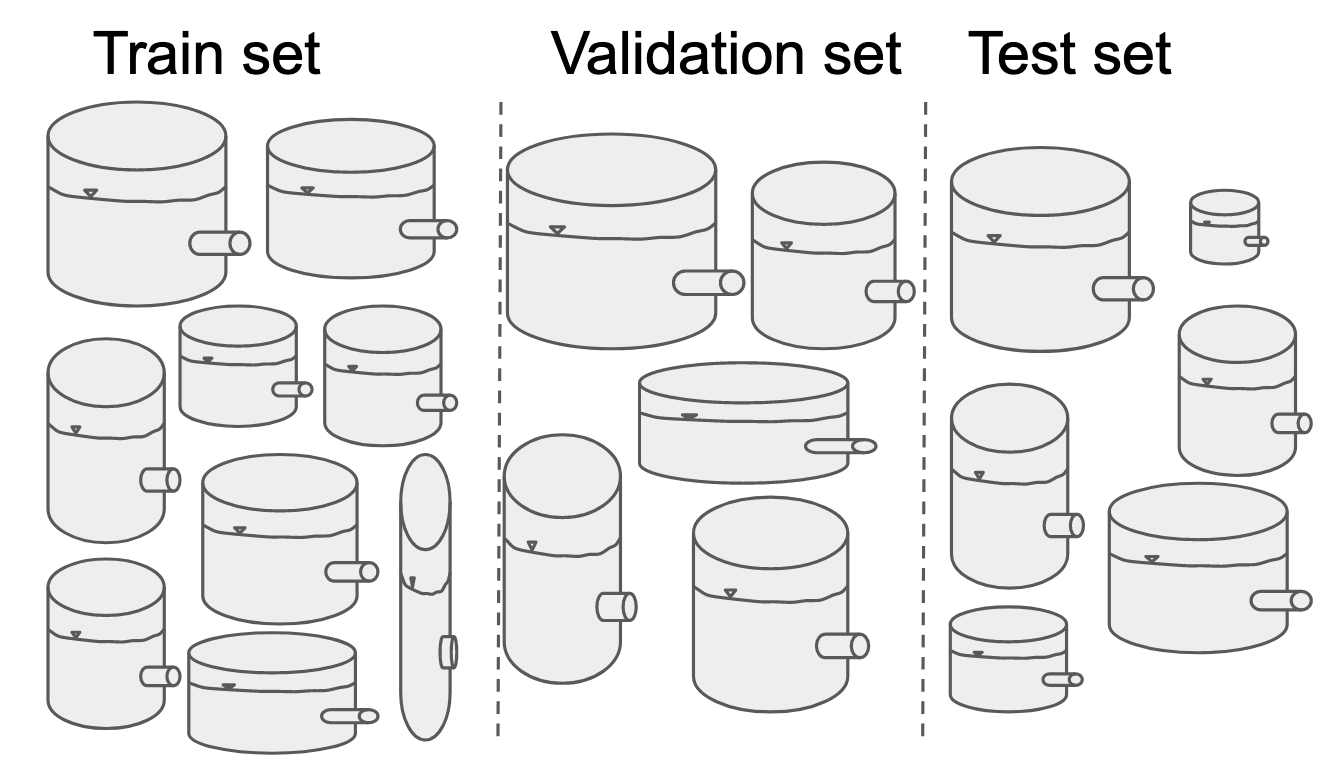
\includegraphics[width=\textwidth]{figures/bucket_splits.png}
\caption{Multiple bucket models representing a basin split into conceptual training, validation, and test sets}
\label{fig:splits}
\end{figure}

% ---------- % ---------- % ---------- % ---------- %
\subsubsection{Training the model: Learning the general response of the example dynamic ''hydrologic" system}
\label{methods:training}

Our intention here is not to attempt to reproduce the well-known and well studied differential equation, but to demonstrate the ability of DeepBucketLab to learn a \emph{general} physical relationship from input and target data. This is often referred to as a "synthetic data experiment''. We chose this particular setup because it provides an intuitive foundation for the same setup often used on ''real-world" experiments, such as \citet{kratzert2019toward, frame2021post, frame2022extreme, frame2023massbalance}.

The training involves using the Adam optimizer, a widely-used algorithm in machine learning that adjusts the model's internal parameters, or 'weights', to enhance its predictions. The training is conducted over several iterations, known as epochs, where the model incrementally improves its understanding of the data. We manage the training data by dividing it into smaller groups, or 'buckets', and using the PyTorch DataLoader for efficient processing. The accuracy of the model's predictions is measured using a custom loss function, which calculates the difference between the model's predictions and the actual target values. After each prediction, the model updates its weights based on the calculated gradients, aiming to reduce the loss in subsequent predictions. We track the training progress visually using the tqdm library, and after each epoch, we calculate the Root Mean Square Error (RMSE), a metric that assesses the model's prediction accuracy. By the end of this training phase, the LSTM model will have learned to predict the dynamics of our synthetic hydrological system, laying the groundwork for applying these techniques to more complex, real-world hydrological data.



% ---------- % ---------- % ---------- % ---------- %
% ---------- % ---------- % ---------- % ---------- %
\subsection{Using neural networks with real world data}
\label{methods:real_world}
In the realm of hydrology, the application of neural networks to real-world data represents a significant leap forward in our ability to model and understand complex hydrological processes. A notable contribution in this field is the work by \cite{Kratzert2022open}, who have developed an extensive neural network package, called NeuralHydrology, specifically tailored for hydrological applications. This package is a valuable resource for researchers and practitioners in the field, offering a range of tools and functionalities that leverage the power of neural networks for hydrological modeling.

One of the key aspects of their work is the inclusion of several tutorials that utilize the CAMELS dataset, as referenced by \citep{Addor2017}. The CAMELS (Catchment Attributes and Meteorology for Large-sample Studies) dataset is a rich collection of hydrological, meteorological, and catchment attributes for over 670 catchments across the United States. It provides a comprehensive and standardized set of data that is ideal for developing and testing hydrological models, including those based on neural networks.

The tutorials included in NeuralHydrology offer practical guidance on applying these advanced modeling techniques to the CAMELS dataset. This not only helps in understanding the nuances of neural network-based hydrological modeling but also provides a hands-on experience in dealing with real-world data. For learners and practitioners new to this field, these tutorials serve as an excellent starting point to explore the capabilities of neural networks in capturing the complexities of hydrological systems.

The integration of neural networks with datasets like CAMELS marks a significant advancement in hydrological sciences. It opens up new possibilities for more accurate and dynamic modeling of hydrological processes.

\section{Experimentation}
\label{methods:experimentation}

The experimentation phase in the DeepBucketLab model is where we explore various scenarios and configurations to understand their impact on the model's behavior and predictions. This phase is integral for gaining deeper insights into the dynamics of our hydrologic system and the capabilities of our LSTM model. It enables us to test hypotheses, explore 'what-if' scenarios, and refine our understanding of the system's responses under varied conditions.

\subsection{Modifying ground truth data and model setup}
In this phase, users are encouraged to experiment with variations in the bucket characteristics and modeling setup. This experimentation can lead to new insights and help in understanding the robustness and adaptability of the model. Here are some ideas for experimentation:

\begin{enumerate}
    \item \textbf{Modifying Ground Truth Data}: 
    \begin{enumerate}
        \item To simulate a more "flashy" system, consider reducing the probability of heavy precipitation and increasing its magnitude. 
        \item For simulating smaller buckets, try reducing the size of the bucket attributes. \item To add more variability, consider increasing the noise level from 0.1 to different values.
    \end{enumerate}

    \item \textbf{Adjusting the Modeling Setup}: 
    \begin{enumerate}
        \item Experiment with the number of training buckets. Increasing or decreasing this number can show how the model performs with more or less training data.
        
        \item Alter the length of the time series. This can help you understand the impact of short-term versus long-term data on the model's learning and predictions.
    \end{enumerate}
\end{enumerate}

\subsubsection{Reconfiguring the Model for New Experiments}
After adjusting the bucket configurations and generating new 'ground truth' data, the next step is to re-create the data loaders for our training, validation, and testing sets. This ensures that our LSTM model is trained and evaluated on the most current and relevant data. The process involves:

    \begin{enumerate}
        \item Re-initializing the bucket configurations with the $setup\_buckets$ function.
        \item Creating new synthetic precipitation data for each bucket.
        \item Running the bucket model simulations again for each bucket.
        \item Visualizing a sample of the bucket fluxes for the validation set.
    \end{enumerate}

Following these steps, we reinitialize the LSTM model and perform the training process with the updated dataset. This reinitialization is crucial to ensure that the model starts with fresh parameters and is capable of learning from the new data without any influence from the previous training sessions.

\subsubsection{Assessing Model Performance Post-Experimentation}
After retraining our LSTM model with the updated dataset, it's important to assess the learning progress and model performance. This is done by:

    \begin{enumerate}
        \item Visualizing the Learning Curve: Plotting the learning curves based on the training results to assess the model's learning efficiency and convergence with the new data.
        \item Validation Check: Evaluating the retrained model's performance on unseen data using the validation set to ensure that it generalizes well.
    \end{enumerate}

These steps are essential for understanding the impact of our experimental changes on the model's learning dynamics and overall performance, thereby providing valuable insights into the system's behavior under these updated scenarios.

% ---------- % ---------- % ---------- % ---------- %
% ---------- % ---------- % ---------- % ---------- %
% ---------- % ---------- % ---------- % ---------- %
% ---------- % ---------- % ---------- % ---------- %
% ---------- % ---------- % ---------- % ---------- %
% ---------- % ---------- % ---------- % ---------- %
\bibliographystyle{unsrtnat}
\bibliography{references}  %%% Uncomment this line and comment out the ``thebibliography'' section below to use the external .bib file (using bibtex) .


%%% Uncomment this section and comment out the \bibliography{references} line above to use inline references.
% \begin{thebibliography}{1}

% 	\bibitem{kour2014real}
% 	George Kour and Raid Saabne.
% 	\newblock Real-time segmentation of on-line handwritten arabic script.
% 	\newblock In {\em Frontiers in Handwriting Recognition (ICFHR), 2014 14th
% 			International Conference on}, pages 417--422. IEEE, 2014.

% 	\bibitem{kour2014fast}
% 	George Kour and Raid Saabne.
% 	\newblock Fast classification of handwritten on-line arabic characters.
% 	\newblock In {\em Soft Computing and Pattern Recognition (SoCPaR), 2014 6th
% 			International Conference of}, pages 312--318. IEEE, 2014.

% 	\bibitem{hadash2018estimate}
% 	Guy Hadash, Einat Kermany, Boaz Carmeli, Ofer Lavi, George Kour, and Alon
% 	Jacovi.
% 	\newblock Estimate and replace: A novel approach to integrating deep neural
% 	networks with existing applications.
% 	\newblock {\em arXiv preprint arXiv:1804.09028}, 2018.

% \end{thebibliography}


\end{document}
